\documentclass[a4paper, 11pt]{article}
\usepackage[a4paper, left=3cm, bottom=4cm, right=3cm]{geometry}

\RequirePackage[english]{babel}
\RequirePackage[utf8]{inputenc}
\RequirePackage{amsmath}
\RequirePackage{amsfonts}
\usepackage{mathtools}
\RequirePackage{hyperref}
\usepackage{tikz}
\usepackage{braket}

\newcommand{\dd}{\mathop{\mathrm{d}\!}{}}
\newcommand{\Tr}{\mathop{\mathrm{Tr}\!}{}}
\newcommand{\deriv}[2]{\dfrac{\dd #1}{\dd #2}}
\newcommand{\pderiv}[2]{\dfrac{\partial #1}{\partial #2}}
\newcommand{\HH}{\mathcal{H}}
\newcommand{\LL}{\mathcal{L}}

\newcommand\braa[1]{{\langle\langle{#1}|}}
\newcommand\kett[1]{{|{#1}\rangle\rangle}}

\renewcommand\bra[1]{{\langle{#1}|}}
\makeatletter
\renewcommand\ket[1]{%
	\@ifnextchar\bra{\k@t{#1}\!}{\k@t{#1}}%
}
\newcommand\k@t[1]{{|{#1}\rangle}}
\makeatother

\bibliographystyle{alpha}

\date{\today}
\author{Bruno Bucciotti}
\title{Quantum information 2}


\begin{document}
	\maketitle
	
	\begin{abstract}
		We restrict our attention to finite dimensional systems.
		
		\href{https://www.youtube.com/watch?v=GyKcdbFGeV8}{90's}
		
	\end{abstract}

	\tableofcontents
	\clearpage
	\section{Lecture}
	Consider a system $S$ coupled to an environment $E$ such that $S+E$ is a closed system described by the Hamiltonian $H_{SE} = H_S + H_E + V_{SE}$, where $H_S,H_E$ stand for $H_S\otimes \hat{1}_E$, $\hat{1}_S\otimes H_E$, and $V_{SE}$ represents an interaction term.
	
	States of $S$ are density matrices $\rho_S\in\sigma(\HH_S)$.
	The time evolution operator is $U_{SE}(t) = \exp^{-i H_{SE} t}$. It maps $\rho_{SE}(0)$ into $\rho_{SE}(t) = U_{SE}(t) \rho_{SE}(0) U^\dagger_{SE}(t)$. Assuming the initial state factorizes into $\rho_S(0)\otimes\tau_E(0)$, we get
	\[ \rho_S(0)\rightarrow \rho_S(t) = \Phi\left[\rho_S(0)\right] = \Tr_E\left[ U_{SE}(t) \left(\rho_S(0)\otimes\tau_E(0)\right) U^\dagger_{SE}(t) \right] \]
	The factorization assumption may seem very restrictive, but actually reflects what happens in the lab, where your state preparation procedure outputs a state for your system which is uncorrelated with the environment, over which we have no control.
	\vspace{5mm}
	
	We proceed to study all such \emph{quantum channels} $\Phi$, holding $t$ and $\tau_E(0)$ fixed.
	
	\noindent First, notice that $\Phi$ is a \emph{superoperator}: it acts a linear transformation on operators on $S$.
	
	\noindent Second, $\Phi$ is defined on \emph{all} linear operators $\mathcal{L}(\HH)$, not just $\sigma(\HH)$; in particular, observables. The extension is trivial
	\[ \Phi\left[\hat{\Theta}\right] = \Tr_E\left[ U_{SE}(t) \left(\hat{\Theta}\otimes\tau_E(0)\right) U^\dagger_{SE}(t) \right] \]
	and it is unique if we require linearity (\emph{proof}: any operator can be decomposed as a linear sum of density matrices). Uniqueness hold even for infinite dimensional systems.
	
	\subsection{Representations of quantum channels}
	\subsubsection{Physical representation}
	The one we just described.
	\subsubsection{Stinespring representation}
	We know we can purify a state by adding extra degrees of freedom. Suppose we purify the state of the environment $\tau_E(0)$ by adding a system $E_1$, $E' = E+E_1$. Then $\tau_E(0) = \Tr_{E_1} \left(\ket{0}_{E'}\bra{0}\right) $. Then, defining $U'_{SE'} = U_{SE} \otimes \hat{1}_{E'}$, we get (simple check)
	\[ \Phi\left[\hat{\Theta}\right] = \Tr_{E'} \left[ U'_{SE'} \left( \hat{\Theta} \otimes \ket{0}_{E'}\bra{0} \right) {U'}^\dagger_{SE'} \right] \]
	
	We have thus proved that the Stinespring representation is not only a special case of physical representation, but equivalent to it. They are both \emph{extrinsic} representations.
	
	\subsubsection{Kraus representation}
	Kraus representation is \emph{intrinsic}, no environment needed. It is defined in terms of a Kraus set $M_k\in \mathcal{L}(\HH_S)$.
	\[ \Phi\left[\hat{\Theta}\right] = \sum_{k=1}^D M_k \hat{\Theta} M_k^\dagger,\qquad \sum_{k=1}^D M_k^\dagger M_k = \hat{1}_S \]
	We already know how to go from Stinespring to Kraus, we now show the other direction.%SHOW ANYWAY
	
	\subsubsection{From Kraus to Stinespring}
	Given a Kraus set $\{M_k\}_{k=1,\dots,D}$, we want to define a system $E$, a unitary $U_{SE}$ and a state $\ket{0}$ s.t.
	\[ \Phi\left[\hat{\Theta}\right] = \Tr_E\left[ U_{SE}(t) \left(\hat{\Theta}\otimes \ket{0}_{E}\bra{0} \right) U^\dagger_{SE}(t) \right] \]
	Start with $E$ s.t. dim$(\HH_E) = D+1$ (actually, $D$ is enough, but the explicit construction is more difficult). Let $\ket{0}$ be any state of $E$ and extend it to an orthonormal basis $\{\ket{k}_{k=0,\dots,D}\}$ of $\HH_E$. Let the evolution be defined by the hamiltonian
	\[ H_{SE} = \omega \sum_{K=1}^{D} M_k\otimes \ket{k}_E\bra{0} + h.c. \]
	Then it's easy to show that for pure states $\ket{\psi}_S$ we get
	\[ \ket{\psi}_S\ket{0}_E \rightarrow \cos(\omega t) \ket{\psi}_S\ket{0}_E - i \sin(\omega t) \sum_{k=1}^{D} M_k \ket{\psi}_S \otimes \ket{k}_E \]
	For $\omega t= \dfrac{\pi}{2}$ we have
	\[ \ket{\psi}_S\bra{\psi} \rightarrow \sum_{k=1}^{D} M_k \ket{\psi}_S\bra{\psi} M_k^\dagger \]
	The extension to the general density matrix case follows from linearity.
	
	\subsubsection{Axiomatic representation}
	We can describe the set of all quantum channels as the set of
	\begin{itemize}
		\item Linear
		\item Completely positive
		\item Trace preserving
	\end{itemize}
	maps. We remind the reader of the definition of complete positivity. Given $\Phi$ superoperator on $S$, $\Phi$ is completely positive if for all ancillas $A$
	\[ (\Phi\otimes \hat{1}_A):\, \mathcal{L}(\HH_S\otimes \HH_A) \rightarrow \mathcal{L}(\HH_S\otimes \HH_A) \]
	is completely positive. Complete positivity implies positivity, but not vice-versa. %GIVE EXAMPLE
	This stronger requirement is necessary when we remember that we can always view any system $S$ as part of a larger system $S+A$, where $A$ maybe is far away and irrelevant.
	
	It is easy to show that all representations fulfill these axioms. We now exhibit an explicit Kraus set for a given channel $\Phi$ satisfying the axioms. To do so, we introduce the Choi-Jamiolkowski isomorphism.
	
	\subsection{Choi-Jamiolkowski construction}
	Given $\Phi$ acting on $S$, we construct an ancilla $A$ with the same dimensionality $d$ (assumed finite, but extensions do exist).
	We first consider any orthonormal basis $\ket{k}_S$, $\ket{k}_A$ and construct
	\[ \ket{\psi_M}_{SA} = \sum_{k=1}^{d} \dfrac{\ket{k}_S\otimes\ket{k}_A}{\sqrt{d}} \]
	maximally entangled state. The Choi state is then defined as
	\[ \rho_{CJ}^\Phi = \left(\Phi\otimes \hat{1}_A\right) (\ket{\psi_M}_{SA}\bra{\psi_M}) \]
	Notice that it is indeed a state. The choice is not unique because we can always change basis. Nevertheless we can now write down a formula (proof by substitutions) for the evolution of any pure state of $S$ in terms of $\rho_{CJ}^\Phi$
	\[ \ket{\psi}_S\bra{\psi} \rightarrow \Phi\left(\ket{\psi}_S\bra{\psi}\right) = d\, \prescript{}{A}{\braket{\psi^* | \rho_{CJ}^\Phi | \psi^*}}_A \]
	where $\ket{\psi^*}_A=\sum \alpha_k^* \ket{k}_A$ if $\ket{\psi}_S=\sum \alpha_k \ket{k}_S$. We can rewrite it as
	\begin{equation}
	\label{eq:1}
	\Phi\left[ \rho_S \right] = d\, \Tr_A\left[ \left(\hat{1}_S \otimes \rho_A^t \right) \rho_{CJ}^\Phi \right]
	\end{equation}
	We immediately see the equivalence when $\rho_S$ is pure (note that $\rho_A^t=\rho_A^*$ due to hermiticity. Note the dependence on the basis chosen to define $\rho_{CJ}$); the extension to generic density matrix $\rho_S$ follows from linearity.
	
	To sum up, $\rho_{CJ}^\Phi$ contains all the information on $\Phi$.
	
	\subsubsection{From axiomatic to Kraus representation}
	Given $\Phi$, construct the Choi state $\rho_{CJ}^\Phi$ and put it in spectral form
	\[ \rho_{CJ}^\Phi = \sum_{\kappa=1}^{d^2} \lambda_\kappa \ket{\kappa}_{SA}\bra{\kappa} \]
	where $\lambda\ge 0$, $\sum \lambda_\kappa = 1$. Substituting in \ref{eq:1} we obtain
	\[ \Phi\left( \ket{\psi}_S\bra{\psi} \right) = d\, \sum \lambda_\kappa \prescript{}{A}{\braket{\psi^*|\kappa}}_{SA} \braket{\kappa|\psi^*}_A \]
	Defining
	\[ \ket{\chi_{l \kappa}}_S \equiv \prescript{}{A}{\braket{l|\kappa}}_{SA} \]
	we get
	\begin{equation}
	\label{eq:2}
	\Phi\left( \ket{\psi}_S\bra{\psi} \right) = d\, \sum \lambda_\kappa \alpha_l\alpha^*_m \ket{\chi_{l\kappa}}_S\bra{\chi_{m\kappa}}
	\end{equation}
	which is \emph{almost} of the form $\sum M_k \ket{\psi}\bra{\psi}M_k^\dagger$. To get there, we further define
	\[ M_\kappa \ket{l}_S  = \sqrt{d\lambda\kappa} \ket{\chi_{l\kappa}}_S \]
	so that from \ref{eq:2} we get
	\[ \Phi\left( \ket{\psi}_S\bra{\psi} \right) = \sum \alpha_l\alpha^*_m M_\kappa \ket{l}_S\bra{m}  M_\kappa^\dagger \]
	Summing over $l,m$ finally results in
	\[ \Phi\left( \ket{\psi}_S\bra{\psi} \right) = \sum_{\kappa=1}^{d^2} M_\kappa \ket{\psi}_S\bra{\psi} M_\kappa^\dagger \]
	The identity
	\[ \Tr_S\left[\Phi\left(\ket{\psi}_S\bra{\psi}\right)\right] = 1 = \sum_\kappa \braket{\psi|M_\kappa^\dagger M_\kappa | \psi} \]
	holds for all $\ket{\psi}$ and shows that $\sum M_\kappa^\dagger M_\kappa = 1$, implying that $\{M_\kappa\}$ is a good Kraus set. Our proof also shows that you can always do with at most $d^2$ Kraus operators, where $d$ is the dimensionality of your system $S$.
	
	\section{Lecture}
	We begin with 2 two observations.
	\paragraph{Upper bounds}
	We observe that unitary evolution $\rho\rightarrow U\rho U^\dagger$ is a CPT map whose Kraus set is singlet $\{U\}$, showing that $d^2$ is \emph{an upper bound} on the \emph{needed} Kraus operators.

	\noindent Further, considering that a Kraus representation $\{M_k\}_{k=1,\dots,D}$ can be converted to a Stinespring representation where the environment has dimension $D$, we deduce that a system of dimensionality $d$ always admits a Stinespring representation with environment at most $d^2$ dimensional.
	\vspace{2mm}
	
	\paragraph{Process tomography}
	In analogy with state tomography, we want an experimental procedure which will allow us to determine the action of some unknown map $\Phi$ with finitely many measurements (to arbitrary accuracy). There are two ways to go.
	\begin{enumerate}
		\item We can appropriately choose $d^2$ states $\{\rho_j\}$, let $\Phi$ act on each and do state tomography. Notice that if we need $n$ copies of a state to determine it with the prescribed accuracy, then $n*d^2$ state preparations (and measurements) will be required.
		\item We can be clever and exploit the Choi state. First, notice that you can prepare it experimentally: you attach an ancilla $A$ to $S$, prepare $\ket{\psi_M}_{SA}$ and let $\Phi$ act on $S$. Then, doing state tomography $n$ times, you determine $\rho_{CJ}^\Phi$ and therefore $\Phi$.
	\end{enumerate}
	The speed-up of the second method relies on our ability to construct a maximally entangled state. This is a first instance of \emph{entanglement as a resource}.
	
	\subsection{Distances on the set of quantum channels}
	We begin with a few remarks on the set $\mathcal{C}(\HH_S)$ of quantum channels on $S$.
	\begin{enumerate}
		\item $\mathcal{C}$ is closed under convex combinations
		\item $\mathcal{C}$ is closed under composition (which is \emph{not} commutative)
		\item Composition gives $\mathcal{C}$ a semigroup structure (remember that noisy channels have no inverse)
	\end{enumerate}
	\vspace{2mm}
	\subsubsection{Trace distance}
	We now introduce our first distance on $\mathcal{C}(\HH_S)$. The idea is to apply $\Phi_{1,2}$ to a state and measure their distance, than take the $\sup$ over all states.
	\[ D_1(\Phi_1, \Phi_2) = \sup_{\rho\in \sigma(\HH_S)} d_1\left( \Phi_1(\rho), \Phi_2(\rho) \right) \]
	where $d_1$ is the trace distance between states. This distance is not very good because entanglement with an ancilla should help distinguish quantum channels (see ref. [4-8] in \href{https://arxiv.org/abs/1004.4110}{Benenti,Strini, 2010}).
	
	\subsubsection{Diamond distance}
	We instead consider the diamond distance $D_\diamond$, defined as
	\[ D_\diamond\left(\Phi_1, \Phi_2 \right) = D_1\left( \Phi_1\otimes \hat{1}_A, \Phi_2 \otimes \hat{1}_A \right) \]
	where $A$ is an ancillary system of dimensionality equal to that of $S$.
	
	\noindent This distance is bounded even when considering multiple copies of the same channel.
	
	We notice that
	\[ D_\diamond(\Phi_1, \Phi_2) \ge d_1\left( (\Phi_1\otimes \hat{1}_A)(\rho_M), (\Phi_2\otimes \hat{1}_A)(\rho_M) \right),\quad \rho_M = \ket{\psi_M}_{SA}\bra{\psi_M} \]
	so
	\[ D_\diamond (\Phi_1, \Phi_2) \ge d_1\left(\rho_{CJ}^{\Phi_1},\,\, \rho_{CJ}^{\Phi_2}\right) \]
	
	\subsubsection{Choi state peculiarity}
	The Choi-Jamiolkowski construction is often dubbed "isomorphism" but, as we will now see, the Choi state $\rho_{CJ}$ possesses some non-trivial properties. Taking the trace over $S$ and making various trivial substitutions results in
	\[ \Tr_S\left[\rho_{CJ}\right] = \dfrac{1}{d} \sum_{j,k=1} \Tr\left[\Phi(\ket{j}_S\bra{k})\right] \ket{j}_A\bra{k} \]
	exploiting the trace preserving property of $\Phi$ we get
	\begin{equation}
	\label{eq:7}
	\Tr_S\left[\rho_{CJ}\right] = \dfrac{1}{d} \sum_k \ket{k}_A\bra{k} = \dfrac{1}{d} \hat{1}_A
	\end{equation}
	Therefore a Choi state reduces to a maximally mixed state on the ancilla.
	
	\subsection{Adjoint channel}
	We know from standard quantum mechanics that we can consider equivalently the Schroedinger picture or the Heisenberg picture. We already generalized the Schroedinger picture to CPT maps $\Phi$, we now want to do the same for the Heisenberg picture.
	\vspace{2mm}
	
	\noindent Working in Kraus representation, $\Phi(\rho) = \sum M_k \rho M_k^\dagger$.
	\[ \braket{O}_{\Phi(\rho)} = \Tr\left[ \hat{O}\, \Phi(\rho) \right] = \Tr\left[\sum_k \hat{O}\, M_k\rho M_k^\dagger \right] =
	\Tr\left[ \left(\sum_k M_k^\dagger \hat{O}M_k\right)\rho \right] \equiv \Tr\left[ \Phi_H \rho \right] \]
	where we defined ($H$ stands for Heisenberg)
	\[ \Phi_H(\hat{O}) = \sum_k M_k^\dagger \hat{O} M_k \]
	
	$\Phi_H$ is called the adjoint channel, because remembering that $\braket{A|B} = \Tr\left[A^\dagger B\right]$ is a scalar product, we get
	\[ \braket{A|\Phi(B)} = \braket{\Phi_H(A)|B} \]
	It is a linear, completely positive super-operator, but it is \textbf{not} trace preserving.
	\[ 1 = \sum M_k^\dagger M_k \neq \sum M_k M_k^\dagger \]
	\noindent Indeed this property is replaced by $\Phi_H(1) = 1$, which is easily verified and goes under the name of \emph{unital property}.
	\vspace{3mm}
	
	The action of $\Phi_H$ in Stinespring representation is left as an exercise, but (my) result is
	\[ \hat{O}_S \rightarrow \prescript{}{E}{\braket{0|U_{SE}^\dagger (\hat{O}_S\otimes \hat{1}_E) U_{SE}|0}_E} \]
	
	\subsection{Complementary channel}
	Consider a Stinespring representation of a quantum channel $\Phi$. We can picture the evolution as a sort of "scattering" of system $S$ in state $\rho$ with system $E$ in state $\ket{0}_E$. The output is of course
	\[ U_{SE} \left(\rho\otimes \ket{0}_E\bra{0}\right) U_{SE}^\dagger \]
	If we trace out $E$ we are left with $\Phi(\rho)$ by definition, but if we trace out $S$ then we are left with a state of $E$. We can therefore define
	\[ \tilde{\Phi}: \sigma(\HH_S)\rightarrow \sigma(\HH_E),\qquad \tilde{\Phi}(\rho) = \Tr_S\left[ U_{SE} \left(\rho\otimes \ket{0}_E\bra{0}\right) U_{SE}^\dagger \right] \]
	This map is easily verified to be linear completely positive and trace preserving. Note that complete positivity means that a positive operator, which (up to rescaling by a positive constant) we can assume to be a density matrix $\rho_{SA}$, gets mapped to a positive operator $\rho'_{AE}$.
	
	There is some freedom in choosing the Stinespring representation, but two different choices leading say to $\tilde{\Phi}$, $\tilde{\Phi}'$ are unitary equivalent, meaning there exist $U,V$ unitary s.t. $\tilde{\Phi}'(\rho) = V \tilde{\Phi}\left( U \rho U^\dagger \right) V^\dagger$ (proof left as an exercise).
	
	Lastly, notice that if we work in physical representation instead of Stinespring then our freedom in choosing the representation is even larger.
	We will end up with $\tilde{\Phi}_W$, $\tilde{\Phi}_W'$ ($_W$ stands for \emph{weak}) not necessarily unitary equivalent. The set of weak complementary channels originating from a given $\Phi$ is considerably harder to study, because different $\tilde{\Phi}$'s represent different physics.
	
	\section{Lecture}
	We begin with a comment on complementary channels from last lecture. Knowing $\Phi(\rho),\tilde{\Phi}(\rho)$ means knowing the two partial traces of the full system $SE$, but we are still missing correlations. Conclusion: $\Phi,\tilde{\Phi}$ contain less information than $U_{SE}$.
	
	\subsection{Degradability}
	We say that a channel $\Phi$ is degradable if there exists $\Lambda:\mathcal{L}(\HH_S)\rightarrow\mathcal{L}(\HH_E)$ LCPT s.t.
	\[ \tilde{\Phi}(\rho) = \Lambda \circ \Phi(\rho) \quad \forall \rho \]
	The physical meaning is that we can \emph{degrade} the state of the system $S$ through some noise and obtain the state of $E$. The state of the environment contains no additional information; $\Phi$ can carry more information than $\tilde{\Phi}$.
	
	\paragraph{Example} $\Phi = \hat{1}_S$ is a degradable channel. Proof: Given $\tilde{\Phi}$ complementary channel of the identity, I claim that $\Lambda = \tilde{\Phi}$ is the right map. It is LCPT and $\tilde{\Phi} = \tilde{\Phi} \circ 1$.
	
	\subsection{Anti-degradability}
	We say that a channel $\Phi$ is anti-degradable if there exists $\Lambda':\mathcal{L}(\HH_E)\rightarrow\mathcal{L}(\HH_S)$ LCPT s.t.
	\[ {\Phi}(\rho) = \Lambda' \circ \tilde{\Phi}(\rho) \quad \forall \rho \]
	Remarks opposite to the previous case hold.
	
	\paragraph{Example} $\Phi(\rho) = \bar{\rho}$. Turn this into a well defined quantum channel (remember the domain is $\mathcal{L}(\HH_S)$, not $\sigma(\HH_S)$), prove LCPT and show that it is anti-degradable.
	
	\emph{Solution} We begin by defining $\Phi(\theta) = \Tr[\theta] \bar{\rho}$. It reduces to the right $\Phi$ on density matrices and it is trace preserving by definition. Linearity being obvious, we are left with complete positivity. Instead of proving it, we take a different route. We can exhibit a Stinespring representation of $\Phi$, that is a unitary $U_{SE}$ s.t., tracing out $E$, $\rho\rightarrow \bar{\rho}$. Then we know that a super-operator $\Phi$ given in Stinespring representation is LCPT.
	
	Write $\bar{\rho} = \sum_{k=1}^{d} \lambda_k \ket{k}_S\bra{k}$, $\lambda_k\ge 0$, $\braket{j|k} = \delta_{jk}$ a basis. We will define $d$ unitary matrices in a moment, but for now let us call them $V_i$. We define $U_{SE}$ on $\ket{k}_S\ket{0}_E$ as
	\[ U_{SE} (\ket{i}_S\ket{0}_E) = \sum_{k=1}^{d} \sqrt{\lambda_k} \ket{k}_S \otimes (V_i\ket{k}_E) \]
	The idea was to write the most general purification of $\bar{\rho}$, where we keep the dependence of $V$ on the input $i$. A unitary extension of $U_{SE}$ to all $\HH_S\otimes \HH_E$ is always possible if we prove
	\[ \prescript{}{E}{\bra{0}} \prescript{}{S}{\bra{i}} U_{SE}^\dagger U_{SE} \ket{j}_S\ket{0}_E = \delta_{ij} \]
	After a few steps we are left with
	\[ \sum_{k} \lambda_k\prescript{}{E}{\braket{k|V_i^\dagger V_j | k}_E} = \delta_{ij} \]
	All is left to do is pick the $d$ unitaries s.t. $\prescript{}{E}{\braket{k|V_i^\dagger V_j | k}_E} = 0$ if $i\neq j$ ($i=j$ is trivial). Observe that
	\[ V_k \ket{i} = \ket{i+k-1 \mod d},\qquad V_k^\dagger\ket{i} = \ket{i+1-k \mod d} \]
	is unitary and satisfies the above requirement.
	
	Finally, $\Phi$ is anti-degradable because $\Phi = \Lambda' \circ \tilde{\Phi}$ holds if we simply pick $\Lambda = \Phi$, which is LCPT as we have just seen.
	
	\subsection{Weak (anti-)degradability}
	Let us extend the concept of (anti)-degradability to the physical representation. Suppose you are given a quantum channel $\Phi$. A channel $\tilde{\Phi}_W$ is called \emph{weak complementary} of $\Phi$ if there are $\tau_E$, $U_{SE}$ s.t.
	\[ \Phi(\rho) = \Tr_E \left[ U_{SE} (\rho\otimes \tau) U_{SE}^\dagger \right],\qquad
	\tilde{\Phi}_W(\rho) = \Tr_S \left[ U_{SE} (\rho\otimes \tau) U_{SE}^\dagger \right] \]
	We say that $\Phi$ is weakly degradable if there is $\Lambda$ LCPT s.t.
	\[ \tilde{\Phi}_W \equiv \Lambda \circ \Phi \]
	and similarly for weak anti-degradability
	\[ \Phi \equiv \Lambda \circ \tilde{\Phi}_W \]
	Propositions:
	\begin{itemize}
		\item anti-degradability is equivalent to weak anti-degradability
		\item degradability implies weak degradability (not vice-versa). W/o proof.
	\end{itemize}
	One implication is easy: take a purification of $\tau_E$, for example $\ket{\phi}_{AE}$ s.t. $\Tr_A\left[ \ket{\phi}\bra{\phi} \right] = \tau_E$. Then $U_{SE}\otimes \hat{1}_A$, $\ket{\phi}_{AE}$ are a Stinespring representation for $\Phi$ with environment AE.
	
	Define
	\[ \tilde{\Phi}_{AE}(\rho) = \Tr_S\left[ (U_{SE}\otimes \hat{1}_A) (\rho\otimes \ket{\phi}_{AE}\bra{\phi}) (U_{SE}^\dagger\otimes \hat{1}_A) \right] \]
	and observe that
	\[ \Phi(\rho) = \Tr_{AE}\left[ (U_{SE}\otimes \hat{1}_A) (\rho\otimes \ket{\phi}_{AE}\bra{\phi}) (U_{SE}^\dagger\otimes \hat{1}_A) \right] \]
	\[ \tilde{\Phi}_W(\rho) = \Tr_{AS}\left[ (U_{SE}\otimes \hat{1}_A) (\rho\otimes \ket{\phi}_{AE}\bra{\phi}) (U_{SE}^\dagger\otimes \hat{1}_A) \right] = \Tr_A\left[\tilde{\Phi}_{AE}(\rho)\right] \]
	If $\Phi$ is degradable, then $\tilde{\Phi}_{AE} = \Lambda \circ \Phi$. Thus we can take the output of $\Phi$, process it with $\Lambda$ and then trace out the ancilla to get $\tilde{\Phi}_W(\rho)$.
	
	\subsection{Compatible channels}
	Two quantum channels $\Phi_1:S\rightarrow S_1$ $\Phi_2:S\rightarrow S_2$ are said to be compatible if there is $\Phi_{12}:S\rightarrow (S_1+S_2)$ s.t.
	\[ \Phi_1(\rho) = \Tr_2\left[\Phi_{12}(\rho)\right],\qquad
	\Phi_2(\rho) = \Tr_1\left[\Phi_{12}(\rho)\right] \]
	Not all channels are compatible, and this language of "compatibility" can be used to rephrase the uncertainty principle and much more.
	
	\paragraph{Example}
	$\Phi$ is an anti-degradable channel iff $\Phi$ and $\tilde{\Phi}$ are compatible. Therefore any non anti-degradable channel can be used to construct two mutually incompatible channels.
	
	\subsection{Spectrum of LCPT maps}
	If there is $\theta\in \mathcal{L}(\HH_S)$ s.t. $\Phi(\theta) = \lambda \theta$, then $\lambda$ is called an eigenvalue of $\Phi$. The set $Sp(\Phi)$ of all $\lambda$'s is called spectrum of $\Phi$.
	
	$\lambda\in Sp(\Phi) \rightarrow \lambda^* \in Sp(\Phi)$. Simply evaluate $\Phi$ of $\theta$ and $\theta^\dagger$ and observe that $(\Phi(\theta))^\dagger = \Phi(\theta^\dagger)$ (use the Kraus form of $\Phi$).
	
	$\forall\, \lambda\in Sp(\Phi)$, $|\lambda|\le 1$. This comes from the contractivity of $\Phi$.
	
	$\forall\,\Phi$ $\lambda=1$ is in the spectrum, that is $\Phi(\theta)=\theta$ always admits a non-zero solution. I attempt a proof (not checked!): either $\Phi$ is not strictly contractive, then it is unitary and any eigenvector evolves with a phase, that is the state is invariant; or $\Phi$ is contractive, then Banach-Caccioppoli theorem guarantees the existence of a fixed point.
	
	\subsection{Ergodic channels}
	Consider a channel $\Phi$ and call $\Phi^2\equiv \Phi\circ\Phi$, $\Phi^3\equiv\dots$ We can imagine a system initialized in a state $\rho$ which evolves in time and becomes $\Phi(\rho),\Phi^2(\rho)\dots$ Consider the sequence
	\[ \sigma_n = \dfrac{\rho + \Phi(\rho) \dots +\Phi^n(\rho)}{n+1} \]
	of the averages. If it converges to some $\rho_0$ $\bf{independent}$ of $\rho$, then the channel is called \emph{ergodic}. A channel is ergodic iff $\lambda=1$ is non-degenerate (if degenerate, the sequence converges to $\theta_1$ or $\theta_2$ depending on the input).
	
	\subsection{Mixing channels}
	Analogously, $\Phi$ is \emph{mixing} if $\Phi^n(\rho)$ converges to some $\bar{\rho}$ independent of $\rho$. Due to Cesaro summation theorem, mixing implies ergodic; the converse is not true. The set of mixing channels is dense in the set of all channels; actually the space of all channels is convex, and the whole bulk is mixing.
	
	\subsection{Liouville space representation}
	We now want to write down matrices for our super-operators In order to do so, we need a way to write operators (on $\HH$) as vectors. To this end, we introduce the notation $\kett{\theta}$.
	\[ \theta = \sum \braket{i|\theta|j} \ket{i}\bra{j},\qquad \kett{\theta} = \sum \braket{i|\theta|j} \ket{i}\ket{j} \]
	What we did was actually introducing a non-canonical isomorphism $\HH\rightarrow \HH^*$ through which we mapped $\HH^*\otimes \HH$ to $\HH^{\otimes 2}$. We give some examples.
	\[ 1 \rightarrow \kett{1} = \sum_{i=1}^d \ket{i}\ket{i} \]
	which is a maximally entangled not-normalized state. It is a simple calculation to show that
	\begin{equation}
	\label{eq:3}
	\kett{\theta} = (\theta \otimes 1) \kett{1} = (1 \otimes \theta^t) \kett{1}
	\end{equation}
	\[ \langle\braket{\theta|\Omega}\rangle = \Tr\left[ \theta^\dagger \Omega \right] \]
	
	\section{Lecture}
	\subsection{Matrix representation for q. channels}
	By making repeated use of identity \ref{eq:3} we deduce the ABC rule
	\begin{equation}
	\label{eq:4}
	\kett{ABC} = (A\otimes C^t)\kett{B}
	\end{equation}
	and from it 
	\[ \kett{\Phi(\theta)} = \kett{\sum_k M_k\theta M_k^\dagger} = \sum_k \kett{M_k \theta M_k^\dagger} = \sum_k (M_k\otimes M_k^*) \kett{\theta} \]
	Thus $M_\Phi = \sum_k M_k \otimes M_k^*$ is a representation of $\Phi$. The spectrum of $\Phi$ is equal to the spectrum of $M_\Phi$. Notice that $M_\Phi$ is not a normal operator, therefore it cannot be diagonalized.
	
	\subsection{Quantum operations}
	We generalize the notion of quantum channel to \emph{quantum operations}: linear completely positive trace reducing maps, that is
	\[ \Lambda\left[\theta\right]\,s.t.\,\Tr\left[\Lambda[\theta]\right] \le \Tr[\theta] \]
	These maps can be physically realized if the true evolution happens in a larger space. Quantum operations admit a (sort of) Kraus decomposition where $\sum_k M_k^\dagger M_k \le \hat{1}_S$.
	
	\subsubsection{POVM}
	We recall some basic facts about POVM, which will play a role shortly.
	
	A POVM is a set $\{E_j\}$ of operators s.t. $\sum E_j = \hat{1}_S$, $E_j\ge 0$. They represent measurements: each $j$ is one possible outcome of the measurement associated with the POVM. How do we use them?
	The probability of outcome $j$ is
	\[ p_j(\rho) = \Tr\left[ E_j \rho \right] \]
	and the state after the measurement is (supposing $j$ came out)
	\begin{equation}
	\label{eq:5}
	\dfrac{U_j \sqrt{E_j} \rho \sqrt{E_j} U_j^\dagger}{p_j}
	\end{equation}
	where $U_j$ depends on the details of the system.
	
	\subsubsection{POVM and quantum operations}
	If we make a measurement on $S$ described by a POVM $\{E_j\}$ and we trash away our knowledge on the outcome, the final state of the system is
	\[ \rho\rightarrow \sum_j p_j \dfrac{U_j \sqrt{E_j} \rho \sqrt{E_j} U_j^\dagger}{p_j} = \sum_j U_j \sqrt{E_j} \rho \sqrt{E_j} U_j^\dagger \]
	This map is a quantum channel (LCPT). If we keep the information on the outcome, then the state is given by \ref{eq:5}. This is not a quantum channel, but it is a quantum operation whose Kraus set is the singlet $U_j\sqrt{E_j}$. Quantum operations are therefore very relevant in measurement theory.
	
	\subsection{Examples of quantum channels}
	\subsection{Unital quantum channels}
	A channel is called unital if $\Phi(\hat{1}_S) = \hat{1}_S$. Put differently, the maximally mixed state is a fixed point. Unitary maps are unital
	\[ \Phi(\rho) = U\rho U^\dagger,\qquad \hat{1}_S \rightarrow \hat{1}_S \]
	Unital channels are $\mathbf{closed}$ under convex combinations.
	
	\subsubsection{Adjoint channel}
	Let us compute the matrix representation of $\Phi_H$. Recall that
	\[ \Tr\left[\theta \Phi(\rho)\right] = \Tr\left[ \Phi_H(\theta) \rho \right] = \langle\braket{\theta|\Phi(\rho)}\rangle = \langle \braket{\theta|M_\Phi|\rho}\rangle = \langle\braket{\Phi_H(\theta)|\rho}\rangle \]
	$\forall\,\rho$, therefore
	\[ \kett{\Phi_H(\theta)} = (M_\Phi)^\dagger \kett{\theta} \]
	Conclusion
	\[ M_{\Phi_H} = (M_\Phi)^\dagger \]
	We note that if $\Phi=\Phi_H$ then the channel is called \emph{self-adjoint}. All self-adjoint channels are unital ($\Phi_H$ are always).
	
	\subsubsection{Qubit channels}
	For qubit unital channels we have the following property
	\[ \Phi(\rho) = \sum p_j U_j \rho U_j^\dagger,\qquad \sum p_j = 1 \]
	Qubit unital channels are convex combinations of unitary transformations. Not true if $d\ge 3$.
	
	Recall that we can represent qubit states as vectors inside the Bloch sphere, that is
	\[ \rho = \dfrac{1+\vec{a}\cdot\vec{\sigma}}{2} \]
	where $|\vec{a}|\le 1$. LCPT maps are from $\rho$ to $\rho'$ or equivalently from $\vec{a}$ to $\vec{a'}$.
	Let us determine $\vec{a'}$ as a function of $\vec{a}$. We abuse notation and write $\Phi(\vec{a})$.
	
	It is straightforward to see that $\Phi(\vec{a})$ must be a linear map, due to linearity of $\Phi$.
	\[ a'_i = T_{ij} a_j + b_i \]
	The trace preserving property is trivial. $\vec{b}$ is the Bloch vector of $\Phi\left(\dfrac{\hat{1}_S}{2}\right)$. If $\Phi$ is unital, then trivially $\vec{b} = 0$.
	
	Complete positivity leads to further constraints, which we will discuss at the beginning of next lecture.
	
	
	\subsubsection{Entanglement breaking channels}
	A channel $\Phi$ on S is entanglement breaking if, for all ancillas A and initial states $\rho_{SA}$
	\[ (\Phi\otimes \hat{1}_A)(\rho_{SA}) = \rho'_{SA} \]
	where $\rho'_{SA}$ is $\mathbf{separable}$. Physically, local noise is capable of destroying all entanglement in the whole system.
	
	The set of all entanglement breaking channels is closed under convex combinations.
	
	Let $\Phi$ be entanglement breaking and $\Phi'$ any channel. Then both $\Phi'\circ \Phi$ and $\Phi\circ \Phi'$ are entanglement breaking. Proof: $\Phi\circ \Phi'$ is trivial; $\Phi'\circ \Phi$ relies on the observation that if you start with no entanglement, local operations cannot create any.
	
	\subsubsection{Shor-Ruskai-Horodecky theorem}
	Any entanglement breaking quantum channel can be effectively described as a crypto-classical channel
	\begin{equation}
	\label{eq:6}
	\Phi(\rho) = \sum_j \rho_j \Tr\left[ E_j \rho \right]
	\end{equation}
	that is, a classical measurement on $\rho$ whose outcome $j$ is used only to determine which $\rho_j$ to prepare, and then $j$ is voided. Stated more precisely, $\Phi$ is entanglement breaking iff there are $E_j$ POVM, $\rho_j$ states s.t. \ref{eq:6} holds. Proof:
	
	We first prove that such a $\Phi$ is entanglement breaking.
	\[ \rho_{SA} \rightarrow \sum_j \Tr_S\left[ E_j \rho_{SA} \right] \otimes \rho_j \]
	where $E_j$ acts on S and $\rho_j$ are states of S. Define
	\[ \tilde{\tau}_j = \Tr_S\left[ E_j \rho_{SA} \right] \]
	It is easy to see that $\tilde{\tau}_j\ge 0$ (mine. check!):
	\[ \braket{\psi|\tilde{\tau}_j|\psi} = \Tr\left[ (E_j\otimes \ket{\psi}\bra{\psi}) \rho_{SA} \right] \ge 0 \]
	where the last inequality comes from observing that that is the probability of finding $\rho_{SA}$ in state $\ket{\psi}_A$ and output $j$ on S in a joint measurement of the two systems. Also
	\[ \Tr_A\left[ \tilde{\tau}_j \right] = \Tr_{SA} \left[ E_j \rho_{SA} \right] = \Tr_S\left[ E_j \rho_S \right] \equiv p_j,\qquad \rho_S = \Tr_A\left[\rho_{SA}\right],\quad \sum_j p_j = 1 \]
	
	Then
	\[ \rho_{SA} \rightarrow \sum_j \tilde{\tau}_j \otimes \rho_j = \sum_j p_j \dfrac{\tilde{\tau}_j}{p_j} \otimes \rho_j \]
	Observing that $\tau_j = \dfrac{\tilde{\tau}_j}{p_j}$ are density matrices we conclude that the final state is separable, hence $\Phi$ is entanglement breaking.
	\vspace{2mm}
	
	We now prove the converse. Given $\Phi$ entanglement breaking, construct $\rho_{CJ}^\Phi$. By definition of CJ state and entanglement breaking
	\[ \rho_{CJ}^\Phi = (\Phi\otimes \hat{1}_A)(\ket{\psi_M}\bra{\psi_M}) = \sum_j p_j\, \rho_j^S\otimes \sigma_j^A \]
	but now we can reconstruct the action of $\Phi$ via the CJ isomorphism
	\[ \Phi(\rho_S) = d \Tr_A\left[ \rho_{CJ}^\Phi (\hat{1}_S\otimes \rho_A^t) \right] = \sum_j p_j\,d\,\Tr_A\left[ \sigma_j^A \rho_A^t \right] \rho_j^S = \sum_j \Tr\left[ p_j\,d\, \sigma_j^t \rho \right] \rho_j^S \]
	All that is left to prove is that $E_j = d\,p_j\,\sigma_j^t$ are a POVM set. They are completely positive (trivially) and
	\[ d\sum_j p_j\,\sigma_j = d \Tr_S\left[ \rho_{CJ}^\Phi \right] = \hat{1}_A \]
	where we used \ref{eq:7} in the last step.
	
	
	\section{Lecture}
	\subsection{Qubit channels constraints}
	We return to qubit channels $\Phi$, where
	\[ \vec{a'} = T\vec{a}+\vec{b} \]
	and we want to constrain $T$ and $\vec{b}$ using complete positivity. We begin with a simpler case: $\Phi$ unitary.
	
	\paragraph{Unitary case} It is well known that the most general unitary 2x2 matrix is 
	\[ U_{\vec{\theta}} = \exp^{-i\frac{\vec{\theta}\cdot\vec{\sigma}}{2}} \]
	up to an irrelevant phase. It can be shown that
	\[ U_{\vec{\theta}} \sigma_i U_{\vec{\theta}}^\dagger = R_{\vec{\theta},\,ij} \sigma_j \]
	Where $R$ is a rotation matrix. Conclusion
	\[ U_{\vec{\theta}} \left(\dfrac{1+\vec{a}\cdot\vec{\sigma}}{2}\right) U_{\vec{\theta}}^\dagger = \dfrac{1+R^{-1}_{\vec{\theta},\,ij} a_j \sigma_i}{2}, \qquad a'_i\rightarrow R^{-1}_{\vec{\theta},\,ij} a_j \]
	where we used the invariance of the scalar product under rotation $R^{-1}$ of both terms.
	\vspace{5mm}
	
	We now exploit unitary equivalence to bring the transformation in a canonical form. Consider $\Phi_1$ unitary equivalent to $\Phi_2$. Let $\Phi_2$ be associated with $T$, $\vec{b}$. Then there are $U,V$ unitaries s.t.
	\begin{equation}
	\label{eq:8}
	\Phi_1(\rho) = U \Phi_2(V\rho V^\dagger) U^\dagger
	\end{equation}
	Let the action of $V$ be associated with a rotation matrix $R_1$; $U$ with $R_2$. Then, proceeding as in the unitary case, \ref{eq:8} becomes
	\[ a'_{\Phi_1(\rho)} = R_2^{-1} \left( T(R_1^{-1} \vec{a}) + \vec{b} \right) = (R_2^{-1}\circ T\circ R_1^{-1}) \vec{a} + R_2^{-1} \vec{b} \]
	Therefore, in the new basis, we have
	\[ T' = (R_2^{-1}\circ T\circ R_1^{-1}),\qquad \vec{b}' = R_2^{-1} \vec{b} \]
	We can always choose (singular value decomposition) $R_1$ and $R_2$ s.t. $T'$ is diagonal
	\[ T' = \begin{pmatrix}
	\lambda_1 & 0 & 0 \\
	0 & \lambda_2 & 0 \\
	0 & 0 & \lambda_3 \\
	\end{pmatrix} \]
	with $\lambda_i$ singular eigenvalues, all $\lambda_i \ge 0$. Any channel is therefore described by six parameters:
	$\lambda_i$ and $\vec{b}$.
	
	
	We state one last result without proof: for $\Phi$ unital ($\vec{b}=0$) the set of allowed $T$ is described by a tetrahedron (interior included) in $\mathbb{R}^3$, where points have coordinates ($\lambda_1,\lambda_2,\lambda_3$). The vertices on the tetrahedron are
	\[ (1,-1,-1)\quad (-1,1,-1)\quad (-1,-1,1)\quad (1,1,1) \]
	All points inside this tetrahedron correspond to LCPT unital quantum channels, all points outside are not completely positive unital maps.
	
	\paragraph{Exercise: amplitude damping} As an exercise, we find $T$ and $\vec{b}$ for an amplitude damping channel.
	%TODOTODOTODO!
	
	\subsection{Gaussian bosonic channels}
	Bosonic channels are typically applied to the electromagnetic field. As such, we need to recall some basic facts about infinite dimensional Hilbert spaces.
	\subsection{Infinite dimensional $\HH$}
	$\HH$ must be separable, that is it must admit a $\mathbf{countably}$ infinite complete set of linearly independent vectors.
	Not all operators on $\HH$ are equally regular: a famous example of the nonsense you get when you're too cavalier about this is
	\[ \Tr\left[ xp - px \right] = \Tr\left[ i\hbar \hat{1}_S \right] \rightarrow 0 = i\hbar\infty?! \]
	We identify the set $\mathcal{B}(\HH) \subset \mathcal{L}(\HH)$ of \emph{bounded} linear operators. These operators have finite norm and are continuous. Further, we identify $\mathcal{B}_1(\HH) \subset \mathcal{B}(\HH)$ the set of \emph{trace class} operators, for which there is a well-behaved notion of trace. The operators are of central interest to us because density matrices are trace 1.
	
	The action of any channel $\Phi$ (and $\Phi_H$) can be extended from $\sigma(\HH)$ to $\mathcal{B}_1(\HH)$, but no further.
	
	\subsection{Harmonic oscillator}
	\emph{Theoretical physics is defined as a sequence of courses each of which deals with the harmonic oscillator. -Sidney Coleman}
	We skip the very basics (introduction of $x,p,H,a,a^\dagger$ operators) and just to displacement operators.
	\subsubsection{Displacement operators}
	\label{subsub:disp.op.}
	\[ D(\mu) = \exp^{\frac{\mu a^\dagger - \mu^* a}{\sqrt{2}}} \]
	CAVEAT: I'M NOT SURE ABOUT $\sqrt{2}$
	
	is a unitary transformation for all $\mu \in \mathbb{C}$. Suppose that the state $\rho$ corresponds to the distribution $f$ in Wigner phase space. Then $D(\mu)$ acts as a rigid displacement
	\[ \rho' = D(\mu) \rho D(\mu)^\dagger \rightarrow f'(x,p) = f(x-\Re(\mu), p-\Im(\mu)) \]
	As a consequence $\braket{x}_{\rho'} = \braket{x}_\rho + \Re(\mu)$, $\braket{p}_{\rho'} = \braket{p}_\rho + \Im(\mu)$.
	
	\subsubsection{Characteristic function} We now introduce the characteristic function $\chi_\rho(\mu)$ of a state $\rho$ as
	\[ \rho = \int \dd^2\mu D(-\mu) \chi_\rho(\mu),\qquad \chi_\rho(\mu) = \Tr\left[D(\mu)\rho\right] \]
	$\chi_\rho(\mu)$ is a complex function of a complex variable and they are in one-to-one correspondence with density matrices.
	
	\subsection{Gaussian states} A state $\rho$ is said to be gaussian when $\chi_\rho(\mu)$ is a gaussian function, that is
	\[ \chi_\rho(\mu) = \exp^{-A|\mu-\mu_0|^2},\quad A> 0 \]
	The Wigner distribution will also be a gaussian function in phase space.
	
	Proposition: $\rho$ is gaussian iff it is a Gibbs state on a quadratic hamiltonian.
	
	\noindent We remind the reader that a Gibbs state is a thermal state
	\[ \rho = \dfrac{e^{-\beta H}}{Z},\qquad Z = \Tr\left[ e^{-\beta H} \right] \]
	As an example, consider a harmonic oscillator with operators $a,a^\dagger$. A Gibbs state would be $\rho_\beta = \dfrac{e^{-\beta\hbar\omega a^\dagger a}}{Z(\beta)}$.
	
	The set of gaussian states is a $\mathbf{non}$-$\mathbf{convex}$ subset of $\sigma(\HH)$. Although mathematically unpleasing, these states are the most common ones we deal with in the lab (especially in quantum optics): laser beams, squeezed laser beams, attenuated or thermalized signals,\dots are all described by gaussian states.
	
	\subsection{Gaussian channels}
	A gaussian channel is any quantum channel with the constraint that gaussian states must be mapped to gaussian states. There is no constraint on the image of non-gaussian states.
	
	Any realistic noise acting on EM field naturally appearing in the lab is going to be represented by the action of a gaussian channel.
	
	\subsubsection{Lossy gaussian channel} We describe the action of the channel on $\chi$ instead of $\rho$.
	Let us focus on one single mode on the EM field.
	\[ \chi_{_{\Phi(\rho)}}(\mu) \equiv \Tr\left[ D(\mu) \Phi(\rho) \right] = \chi(\sqrt{\eta}\mu) \exp\left[-(1-\eta) \frac{|\mu|^2}{2} \right] \]
	where $\eta\in[0,1]$ is a characteristic parameter of the channel $\Phi$. $\eta=1$ means no loss; $\eta=0$ means complete loss of information and energy.
	
	\subsubsection{Beam splitter}
	Beam splitters \ref{fig:bs} are a very common piece of apparatus routinely used in quantum optics experiments.
	They are the perfect place to start if we want to put our new definitions in practice. We will now realize a lossy gaussian channel $\Phi$ with a beam splitter.
	
	\begin{figure}
		\centering
		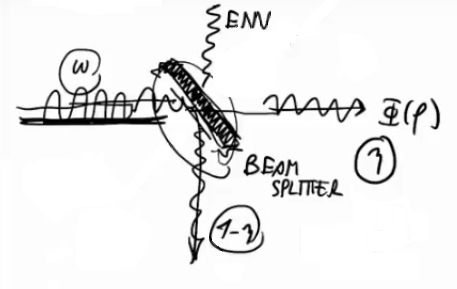
\includegraphics[width=0.7\linewidth]{BS}
		\caption{Beam splitter}
		\label{fig:bs}
	\end{figure}
	We focus our attention on one single frequency $\omega$. We send in a signal from the left onto the beam splitter (B.S.). A fraction $\eta$ (called \emph{transmission coefficient}) of the energy is transmitted; a fraction $1-\eta$ is reflected down. The environment plays an active role even if it is in the vacuum state $\ket{0}_E$. Indeed the action of the beam splitter can be described by some unitary s.t.
	\[ \Phi(\rho) = \Tr_E\left[U (\rho\otimes \ket{0}_E\bra{0}) U^\dagger \right] \]
	
	\section{Lecture}
	\subsubsection{Thermal channel}
	This is another example of a sigle mode bosonic gaussian map. It is defined as
	\[ \chi_{\rho'}(\mu) = \chi(\sqrt{\eta}\mu) \exp^{-(1-\eta)(N+\frac{1}{2}) |\mu|^2} \]
	where $\eta$ and $N$ are parameters describing the channel. $N\ge 0$ is related to the temperature of the environment by the following
	\[ N = \dfrac{1}{e^{\beta\omega} -1} \]
	The physical representation of the channel is described in figure \ref{fig:thermal}. The environment is in a Gibbs state of inverse temperature $\beta$. Some of the input photons are reflected out, while some of the thermal photons from the environment are reflected into the output. In the limit $\beta\rightarrow \infty$ we recover the lossy gaussian channel.
	
	\begin{figure}
		\centering
		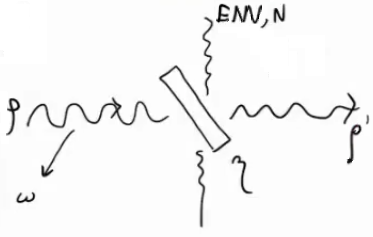
\includegraphics[width=0.7\linewidth]{thermal}
		\caption{}
		\label{fig:thermal}
	\end{figure}
	
	\subsection{Multi-mode extension}
	\subsubsection{QFT recap}
	We recall some basic quantum electrodynamics. The (operator) vector potential $A$ can be decomposed in annihilation and creation operators. The field decomposes in an infinite set of quantum harmonic oscillators. We neglect polarization for simplicity and put the system in a box.
	\[ A(x,t) = \sum_p \dfrac{1}{\sqrt{2\omega_p}} (a_p e^{-ipx} + a_p^\dagger e^{ipx}) \]
	\[ [a_p, a_q^\dagger] = \delta_{p,q} \]
	
	\subsubsection{Symplectic group}
	Given that the electromagnetic degrees of freedom can be represented as $n$ ($n$ is actually infinite) harmonic oscillators, we introduce
	$q^1,p_1,q^2,p_2,\dots,q^n,p_n$ and
	\[ \vec{R} = (q^1,q^2,\dots,q^n;p_1,p_2,\dots,p_n) \]
	which can be used to summarize the commutation relations as
	\[ [R_i, R_j] = i (\sigma_{2n})_{ij} \]
	\[ \sigma_{2n} = \begin{pmatrix}
	0 & \hat{1}_{n _xn} \\
	-\hat{1}_{n _xn} & 0 \\
	\end{pmatrix} \]
	where $\sigma_{2n}$ is the \emph{commutation matrix} of the model. We give some properties of $\sigma_{2n}$
	\[ \det \sigma_{2n} = 1,\qquad \sigma_{2n}^t = \sigma_{2n}^{-1} = -\sigma_{2n} \]
	\vspace{2mm}
	
	\noindent The matrix transformations which preserve $\sigma_{2n}$ are called \emph{symplectic}:
	\[ S\sigma_{2n} S^t = \sigma_{2n} \]
	and they form the \emph{symplectic group}. It is easy verified that $S=1$ is symplectic and that if $S$ is symplectic then $S^{-1}$ is as well. Taking the inverse, we also prove that $S^t$ is symplectic.
	\[ \sigma_{2n} = S\sigma_{2n}S^t \rightarrow \sigma_{2n}^{-1} = S^{-1t}\sigma_{2n}^{-1} S^{-1} \rightarrow \sigma_{2n} = T^t \sigma_{2n} T,\quad T = S^{-1} \]
	where $T$ is any symplectic matrix, because $S^{-1}$ is.
	
	\subsubsection{Weyl displacement operator}
	Consider a list of $2n$ real parameters
	\[ \vec{z} = (x_1,x_2,\dots,x_n;y^1,y^2,\dots,y^n) \]
	We can associate to any $z$ a \emph{Weyl displacement operator}
	\[ V(z) = e^{i\vec{R}\cdot \vec{z}} \]
	Noting that $\vec{R}_i$ is hermitean and that $\vec{z}_i$ is real, we deduce that $V(z)$ is a unitary operator. It can be viewed as a linear combination of creation and annihilation operators, much like $A$.
	
	\noindent If $n=1$ then we are considering a single mode and we are back to \nameref{subsub:disp.op.}. Constructions performed with single mode displacement operators generalize to the multi-mode case.
	
	\subsubsection{Metaplectic representation and trivial generalizations}
	
	\paragraph{Theorem}
	Suppose $U$ unitary is a canonical transformation, meaning $U R_j U^\dagger = M_{jj'} R_{j'}$, $M$ invertible.
	The action of $U$ preserves the commutation relations
	\[ [UR_iU^\dagger, UR_jU^\dagger] = U [R_i, R_j] U^\dagger = i U (\sigma_{2n})_{ij} U^\dagger = i (\sigma_{2n})_{ij} \]
	and defines an action on $V(z)$. Moreover
	\[ UV(z)U^\dagger = e^{i (UR_jU^\dagger) z_j} = e^{i z_j M_{jj'} R_{j'}} = e^{i z'_{j'} R_{j'}}=V(z'),\quad z'_{j} = M^t_{jj'} z_{j'} \]
	
	(Metaplectic stuff..?). We can go the other way: given a transformation $z\rightarrow z'=Mz$ (M invertible) we can interpret it as arising from a canonical transformation.
	
	\paragraph{Characteristic function (again)}
	The multidimensional characteristic function is defined as
	\[ \chi_\rho(z) = \Tr\left[ \rho V(z) \right] \]
	\[ \rho = \int \dfrac{\dd^{2n} z}{(2\pi)^n} V(z) \chi_\rho(z) \]
	CAVEAT: $(2\pi)^n$ or $(2\pi)^{2n}$?
	\paragraph{Gaussian state}
	$\rho$ is gaussian if $\chi(z)$ is gaussian in its $2n$ real parameters. We can always write
	\[ \chi(z) = \exp\left[ -\frac{1}{4} z^t \gamma z - i\vec{m}\cdot\vec{z} \right] \]
	where $\gamma$ is positive semidefinite. It can be shown that the displacement vector $m$ is given by
	\[ \vec{m} = \Tr[\rho \vec{R}] \]
	while the covariance matrix $\gamma$ is
	\[ \gamma = \Tr\left[ \rho \{R_j-m_j\,1, R_{j'}-m_{j'}\,1\} \right],\quad {A,B} \equiv AB+BA \]
	Intuitively $\vec{m}$ is the vector of the average values of positions and momenta; $\gamma$'s diagonal elements are the variances, while the off diagonal terms are the correlations.
	
	From the Heisenberg uncertainty principle it can be shown that not only $\gamma\ge 0$, but also
	\[ \gamma \ge i \sigma_{2n} \]
	Finally, observe that $\gamma$ and $\vec{m}$ can be defined for any state, but gaussian states are $\mathbf{uniquely}$ identified by their $\gamma$ and $\vec{m}$. Indeed, given $\gamma \ge i \sigma_{2n}$ and $\vec{m}$ there is a unique gaussian state.
	
	\subsubsection{Williamson theorem}
	Williamson theorem provides us with a canonical form for $\gamma$ covariance matrix (for any state, even nongaussian). The most general matrix fulfilling $\gamma\ge i \sigma{2n}$ is given by
	\[ \gamma = S\begin{pmatrix}
	D_{n _x n} & 0 \\
	0 & D_{n _x n} \\
	\end{pmatrix} S^t \]
	where $S$ is a symplectic matrix and
	\[ D_{n _x n} = \begin{pmatrix}
	d_1 & 0 & \dots \\
	0 & d_2 & \dots \\
	\dots
	\end{pmatrix} \]
	that is $D$ is diagonal, and $d_k\ge 1$ are called \emph{symplectic eigenvalues}.
	
	It can be shown (exercise!) that $d_k$'s are the eigenvalues of $M = -\sigma_{2n} \gamma \sigma_{2n}\gamma$.

	\noindent Proof: Substituting $\gamma = S\begin{pmatrix}
	D_{n _x n} & 0 \\
	0 & D_{n _x n} \\
	\end{pmatrix} S^t$ in the definition of $M$ and putting $Mv = \lambda v$, $w = S^t v$, we have that the eigenvectors are $v = S^{-1t} \bar{w}$, where $\bar{w}$ is a vector in the canonical basis of $\mathbb{R}^{2n}$. The eigenvalue is $d_k^2$.
	
	\noindent CAVEAT: the claim looks false, and indeed M is quadratic in D, so it makes sense that applying $M$ results in factors $d^2$ (while we would like linear $d_k$).
	
	\paragraph{Theorem} As in the single mode case, $\rho$ is gaussian iff it is a Gibbs state of some hamiltonian quadratic in the field variables $H = \sum c_{jj'}R_jR_{j'}$.
	
	\paragraph{Gaussian channel}
	The extension to the multi-mode case is trivial to define. The most general gaussian channel can be written as
	\[ \chi_{\rho'}(z) = \chi_\rho(Xz) \exp\left[ -\frac{1}{2} z^tYz + i\vec{v} \cdot \vec{z} \right] \]
	where $\vec{v}$ is free of constraints and $X,Y$ are matrices s.t.
	\[ Y \ge i (\sigma_{2n} - X^t \sigma_{2n} X) \]
	
	\subsection{Continuous time evolution in open quantum systems}
	Up till now we discussed the most general transformation the system can undergo in a fixed time $t$. We now turn to the problem of describing the dynamics of the system in time. This is a generalization to open quantum systems of the Schroedinger equation
	\[ \dot{\rho}(t) = -\frac{i}{\hbar} [H, \rho(t)] \]
	The first point is that information can flow in and out of the system and the environment, making it impossible to write down a dynamical equation involving only the degrees of freedom of the system. We will therefore specialize to special environments.
	
	\paragraph{Time dependent hamiltonians} As an aside, we recall that for closed systems $H$ can in general be time dependent (e.g. turn gates on and off, external fields, $H$ time independent but we go in interaction picture). In that case, Schroedinger equation still holds, but
	$U(t)=e^{-i H t}$ is replaced by Dyson time ordered exponential
	\[ U(t,0) = \mathcal{T}\exp\left[-\frac{i}{\hbar} \int_{0}^{t} H(t') \dd t' \right] \]
	
	\paragraph{Divisibility} It is obvious that
	\[ U(t_2, t_0) = U(t_2, t_1) U(t_1, t_0)\quad \forall t_2\le t_1 \le t_0 \]
	that is we can divide time evolution in any number of steps. This property holding for all times $t_2, t_0$ is equivalent to $U$ satisfying a linear differential equation. Because we argued that there is no linear dynamical law for generic environments, it follows that divisibility is generally lost in open quantum system dynamics.
	
	\section{Lecture}
	\subsection{Divisibility}
	\subsubsection{Connecting channel}
	Let's go back to the question of divisibility for a family of channels $\{\Phi(0\rightarrow t)\}_t$. We want to know if, given two elements of the family, there is a LCPT \emph{connecting} channel $\Lambda$ s.t.
	\[ \Phi(0\rightarrow t) = \Lambda(t'\rightarrow t) \circ \Phi(0\rightarrow t') \]
	
	\subsubsection{Factorizable case}
	We work in physical representation and introduce the superoperator $\mathcal{U}$ as a shorthand notation for time evolution
	\[ \mathcal{U}(0\rightarrow t) (\theta) = U_{SE}(0\rightarrow t)\, \theta\, U_{SE}^\dagger(0\rightarrow t) \]
	Assume that at time $t'$ the state of the system+environment can be written as
	\[ \mathcal{U}(0\rightarrow t')(\rho_S(0)\otimes \tau_E(0)) = \rho_S(t')\otimes \tau_E(t') \]
	Then
	\[ \Phi(0\rightarrow t')(\rho_S(0)) = \rho_S(t') \]
	If $\tau_E(t')$ does not depend on $\rho_S(0)$ then we can write down a $\Lambda$ connecting channel as
	\[ \Lambda(t'\rightarrow t)(\theta) = \Tr_E\left[ \mathcal{U}(t'\rightarrow t) (\theta\otimes \tau_E(t')) \right] \]
	$\Lambda$ is LCPT because we are exhibiting a physical representation for it. In general, though, the state at time $t'$ will not factorize, so our construction is not very applicable.
	
	\subsubsection{General proof of non-divisibility (sketch)}
	We are looking for $\Lambda$ s.t.
	\[ \Phi(0\rightarrow t) = \Lambda(t'\rightarrow t) \circ \Phi(0\rightarrow t') \]
	Remembering that non-maximal rank matrices are a set of measure zero, that is any map is arbitrarily close to an invertible map, we can write a formal inverse of $\Phi$ and define $\Lambda$ as
	\[ \Lambda(t'\rightarrow t) = \Phi(0\rightarrow t) \circ \Phi^{-1}(0\rightarrow t') \]
	where $\Phi^{-1}$ will not in general be LCPT, but simply the mathematical inverse.
	
	We immediately see that $\Lambda$ is linear and trace preserving, but we claim that almost always it will not be completely positive.
	To check that we may consider the Choi isomorphism and check if the Choi operator $\theta_{CJ}^\Lambda$ is positive semidefinite
	\[ (\Lambda(t'\rightarrow t)\otimes \hat{1}_A) (\ket{\psi_M}\bra{\psi_M}) = \theta_{CJ}^\Lambda \ge 0 \]
	(we remind the reader that $\Lambda$ is LCPT \emph{iff} $\theta_{CJ}^\Lambda \ge 0$). We won't show this, but claim that this almost never happens.
	
	\subsection{Recovering divisibility}
	We now describe a seemingly special kind of environment which is actually quite common and interesting. We describe the approximations we make along the way.
	\subsubsection{Structured environment}
	Assume that the environment is separable into a \emph{local environment} and a \emph{distant environment}. The system is coupled to the local environment, which in turn interacts with the (much larger) distant environment.
	
	The interaction of local and distant environment has the net effect of resetting the state of the local environment into a given state $\tau_{E_L}$ (imagine that the distant environment is a thermal bath resetting the local environment into a Gibbs state of specified temperature).
	
	Suppose further that all our measurements are coarse-grained, meaning that they last for some characteristic time $\tau$ longer that the typical time scale of the interaction of local and distant environment. We then measure the averaged density matrix $\frac{1}{\tau} \int_{t}^{t+\tau} \rho(t')\,\dd t'$. Under these assumptions divisibility is effectively recovered. This is not a proof, that will come next time.
	
	\subsection{Divisibility criteria}
	We begin by defining precisely what we mean by divisibility
	\paragraph{Def: divisibility} A family $\{\Phi(0\rightarrow t)\}_t$ is said to be divisible if $\forall\,t, t'\le t$ there is $\Lambda(t'\rightarrow t)$ connecting channel LCPT s.t. $\Phi(0\rightarrow t) = \Lambda(t'\rightarrow t) \circ \Phi(0\rightarrow t')$.
	
	\paragraph{Def: positive divisibility} Same definition but now $\Lambda$ is only required to be linear positive and trace preserving. It is clear that positive divisibility, lacking complete positivity, has no physical meaning in general and that it is implied by divisibility. The trace distance criterion below will illustrate why this definition was introduced at all.
	\vspace{4mm}
	
	Given a family $\{\Phi(0\rightarrow t)\}_t$, we want to find necessary and/or sufficient conditions for it to be divisible. We will give only one instance of such criteria, but there are more in the literature.
	\subsubsection{Trace distance}
	We know that the trace distance between two states cannot expand during a physical time evolution. Therefore, fixing $t$, $t'\le t$ and two states $\rho(0),\sigma(0)$ of S, we trivially have
	\[ D(\sigma(t), \rho(t)) \le D(\sigma(0), \rho(0)),\qquad D(\sigma(t'), \rho(t')) \le D(\sigma(0), \rho(0)) \]
	If the family is divisible, then also
	\[ D(\sigma(t), \rho(t)) \le D(\sigma(t'), \rho(t'))  \]
	that is, $D(\sigma(t), \rho(t))$ is monotonically non-increasing. Unfortunately even positive divisible families have this property, so we can immediately tell that the condition is necessary (for $\{\Phi\}_t$ to be divisible) but not sufficient.
	
	\subsection{Relation with markovianity}
	We give all definitions as if time were discrete. Generalization to continuous time is straightforward.
	\paragraph{Def: random process} A random process is a sequence of outcomes for some event. The outcomes are labeled in time as $x_1,x_2,\dots,x_n$. There is a notion of probability for any sequence of outcomes $P(x_1,x_2,\dots,x_n)$ (\emph{joint probability}). There is also a notion of \emph{conditional probability} $P(x_n|(x_1,\dots,x_{n-1})) = \dfrac{P(x_1,\dots,x_{n-1},x_n)}{P(x_1,\dots,x_{n-1})}$. The conditional probability acts as a sort of dynamical law of evolution: it maps states (probability distributions) into other states forward in time.
	
	\paragraph{Def: markovian random process} 
	A random process is \emph{markovian} if the conditional probability of the $n-th$ outcome depends only on the $(n-1)-th$ outcome.
	\[ P(x_n|(x_1,\dots,x_{n-1})) \equiv P(x_n|x_{n-1}) \]
	We say that the system has no memory. It is clear that a markovian random process is divisible (just apply the conditional probability law of evolution to get $\Lambda$).
	
	A divisible random process is markovian (define $P(x_n|x_{n-1}$ as the probability of outcome $x_n$ when applying $\Lambda(t_{n-1}\rightarrow t_n)$ to a distribution centered at $x_{n-1}$).
	
	Therefore we will use markovian and divisible interchangeably.
	
	\paragraph{Example}
	Consider Rabi oscillations of an atom trapped in an electromagnetic cavity. The system S (atom) can either be in the ground state or in a particular excited state of energy $\omega$, and the electromagnetic modes allowed in the cavity have been reduced to a single one of same frequency $\omega$.
	
	\noindent We can define time evolution for the atom by tracing away the cavity. The family $\{\Phi\}_t$ generated in this way is clearly not divisible: the system state oscillates from the initial state to the ground state.
	
	However, if we allow leaks of energy from the cavity (local environment) to the outside world (distant environment) then, assuming enough dissipation, the state of the atom will simply flow to the ground and the evolution will become markovian.
	
	\section{Lecture}
	\subsection{Master equation}
	\subsubsection{Dynamical semigroup}
	Given $\mathcal{F} = \{\Phi(0\rightarrow t)\}_t$ divisible, we say that it is a \emph{dynamical semigroup} if the connecting superoperator is homogeneous in time (i.e. it depends only on $t'-t$).
	
	\subsubsection{Master equation}
	If the evolution is governed by a dynamical semigroup, $\rho$ obeys a first order differential equation called \emph{master equation}
	\[ \dot{\rho}(t) = \LL\left[ \rho(t) \right] \]
	where $\LL$ is the \emph{Lindblad} superoperator (also called $GKSL$ superoperator). We proceed to give a general form of this superoperator.
	\[ \LL[\hat{\theta}] = -i \left[H, \hat{\theta}\right] + \mathcal{D}[\hat{\theta}] \]
	where $H$ is the \emph{effective hamiltonian} (hermitean) and $\mathcal{D}$ is called the \emph{dissipator}. $\mathcal{D}$ can always be written using a set of operators called \emph{Lindblad operators} $\{ L_k \}_k$ as
	\[ \mathcal{D}[\theta] = \sum_k \left(2 L_k\theta L_k^\dagger - L_k^\dagger L_k \theta - \theta L_k^\dagger L_k \right) \]
	We claimed that for any dynamical semigroup there is a $\LL$ superoperator, but the converse is also true, provided $\LL$ is of the form given above (there are no restrictions on $\{L_k\}$).
	
	We will now prove that, given a dynamical semigroup, we can write down a master equation. Next lecture we will give a microscopic derivation of the master equation starting from a physical representation system+environment.
	
	\subsubsection{From dynamical semigroup to $\LL$}
	We are given a dynamical semigroup family $\mathcal{F}$ of superoperators. Time homogeneity implies ($t \ge t'$)
	\[ \Phi(t) = \Lambda_{t-t'} \circ \Phi(t') \]
	and, putting $t'=0$, it is easily shown that
	\[ \Lambda_{t-t'} = \Phi(t-t') \]
	We begin by observing that
	\[ \dot{\rho}(t) = \lim_{\epsilon\rightarrow 0^+} \dfrac{\rho(t+\epsilon)-\rho(t)}{\epsilon} = \left(\lim_{\epsilon\rightarrow 0^+}
	\dfrac{\Phi(\epsilon)-1}{\epsilon}\right) \rho(t) \equiv \LL[\rho(t)] \]
	We now have to show that $\LL$ can be cast in the form detailed above.
	
	First, consider a Kraus decomposition $\{M_k(t)\}$ for $\Phi(t)$ at any given $t$. It can be shown that, because we assume $\Phi(t)$ to be differentiable, each element of the Kraus set is differentiable.
	
	We introduce a basis $\{\hat{F}_k\}_{k=0\dots (d^2-1)}$ for the $d$ dimensional space of linear operators on $\HH_S$.
	Then we can decompose each element of the Kraus set as
	\[ M_l(t) = \sum_{k=0}^{d^2-1} C_{lk}(t) \hat{F}_k \]
	We assume $\hat{F}_0 = \hat{1}$. Then $C_{lk}(0) = \delta_{k,0}$. By substitution it is easy to show that
	\[ \LL[\theta] = \deriv{\Phi}{t}(t=0) [\theta] = \deriv{}{t} \sum_{k,k'=0}^{d^2-1} \left( \sum_l C_{lk}(t) C_{lk'}^*(t) \right)|_{t=0} \hat{F}_k \theta \hat{F}_{k'}^\dagger \]
	\[ = \sum_{k,k'} \dot{\chi}_{k,k'}(0) \hat{F}_k \theta \hat{F}_{k'}^\dagger,\qquad \chi_{k,k'}(t) = \sum_l C_{lk}(t) C_{lk'}^*(t) \]
	$\chi_{k,k'}(t)$ is a $d \times d$ positive semidefinite matrix. For generic $t$, its derivative can only be proven to be hermitean.
	
	We now split the sum over $k,k'$ in four pieces
	\[ \LL[\theta] = 2 \dfrac{\dot{\chi}_{00}(0)}{2} \hat{1}\theta \hat{1} + \sum_{k=1} \dot{\chi}_{0k}(0) \hat{1} \theta \hat{F}_k^\dagger +
	\sum_{k=1} \dot{\chi}_{k0}(0) \hat{F}_k \theta \hat{1} + \sum_{k,k'=1} \dot{\chi}_{kk'}(0) \hat{F}_k \theta \hat{F}_{k'}^\dagger \]
	Rearranging we get
	\[ \LL[\theta] = \hat{A} \theta + \theta \hat{A}^\dagger + \sum_{k,k'=1}^{d^2-1} \dot{\chi}_{kk'}(0) \hat{F}_k \theta \hat{F}_{k'}^\dagger,\qquad	\hat{A} = \dfrac{\dot{\chi}_{00}(0)}{2} \hat{1} + \sum_{k=1} \dot{\chi}_{k0}(0) \hat{F}_k \]
	
	Considering $\dot{\rho}(t) = \LL[\rho(t)]$, taking the trace and using linearity to argue $\Tr[\dot{\rho}]=0$ we deduce
	\[ \Tr\left[ \LL[\hat{\theta}] \right] = 0 \]
	where $\hat{\theta}$ is any operator, not just a density matrix, because any $\hat{\theta}$ can be decomposed in terms of density matrices and all equations are linear. Substituting our expression for $\LL[\theta]$ and using the ciclicity of the trace we obtain
	\[ \Tr\left[ \left(\hat{A} + \hat{A}^\dagger + \sum_{kk'=1} \dot{\chi}_{kk'}(0) \hat{F}_{k'}^\dagger \hat{F}_k\right) \hat{\theta} \right] = 0,\quad \forall\, \hat{\theta} \]
	Because $\Tr[AB^\dagger]$ is a non-degenerate scalar product, we deduce that the operator in parenthesis is identically zero. We deduce
	\[ \hat{A} + \hat{A}^\dagger = - \sum_{kk'=1} \dot{\chi}_{kk'}(0) \hat{F}_{k'}^\dagger \hat{F}_k \]
	We have therefore fixed the hermitean part of $\hat{A}$; the anti-hermitean part is unconstrained. Calling it $-iH$, we can write
	\[ \hat{A} = -\frac{1}{2} \sum_{kk'=1} \dot{\chi}_{kk'}(0) \hat{F}_{k'}^\dagger \hat{F}_k - i\hat{H} \]
	
	Substituting $\hat{A}$ into $\LL$ we almost get what we want. The essential problem is that we still have a double summation over $k,k'$ from 1 to $d^2-1$. To solve that, we will diagonalize the submatrix $\xi_{kk'} = \dot{\chi}_{kk'}(0)$, $k,k'\ge 1$, by first showing that $\xi$ is positive semidefinite.
	\[ \xi_{kk'} = \dot{\chi}_{kk'}(0) = \lim_{\epsilon\rightarrow 0^+} \dfrac{\chi_{kk'}(\epsilon) -\chi_{kk'}(0)}{\epsilon} =
	\lim_{\epsilon\rightarrow 0^+} \dfrac{\chi_{kk'}(\epsilon)}{\epsilon} \]
	where in the last step we used that, for $k,k'\ge 1$, $\chi_{kk'}(0)=0$ (by definition, using $C_{lk}(0)=\delta_{k,0}$).
	$\chi_{kk'}(\epsilon)\ge 0$ for any $\epsilon$, therefore $\xi\ge 0$. Diagonalizing $\xi = UDU^\dagger$ and defining
	\[ L_j = \sqrt{D_{jj}} \sum_{k=1} \frac{U_{kj}}{2} \hat{F}_k,\qquad L_j^\dagger = \sqrt{D_{jj}} \sum_{k=1} \frac{U^\dagger_{jk}}{2} \hat{F}^\dagger_k \]
	we (at last) get the desired form for $\LL$.
	
	\section{Lecture}
	\subsection{Fixed point state}
	We show that $0$ is an eigenvalue of $\LL$. Consider the Liouville representation
	\[ \kett{\LL[\theta]} = M_\LL \kett{\theta} \]
	We already proved that $\langle\braket{\hat{1}|\theta}\rangle = \Tr[\theta]$ and that $\Tr[\LL[\rho]] = 0$. Therefore
	\[ \langle \braket{\hat{1}|M_\LL|\theta}\rangle = 0,\quad \forall\,\theta \]
	Thus $\langle\braa{\hat{1}}$ is a left eigenvector with eigenvalue 0. 0 is also a right eigenvalue (just linear algebra), but because $M_\LL$ is not normal, we don't know what the corresponding eigenvector is. It can be shown that it can be chosen to be a density matrix (?positivity?notanexercise).%TODO
	This state $\rho_0$ is a fixed point in the dynamics (generically unique).
	
	\subsection{Solving the L. equation and Adjoint}
	
	\paragraph{Integrating the Lindblad equation}
	The solution is
	\[ \rho(t) = e^{\LL t} \rho(0) \]
	
	\paragraph{Adjoint}
	Recall that in the Heisenberg picture observables evolve, while states do not. We can write a differential equation for the adjoint of $\Phi_t$, if we define $\LL^{(H)}$ as the adjoint of $\LL$.
	\[ \braket{A}_t = \Tr[A\Phi_t(\rho(0))] \]
	\[ \dot{\braket{A}}_t = \Tr\left[ A \LL[\rho(t)] \right] = \Tr\left[ \LL^{(H)}[A] \rho(t) \right] = \Tr\left[ \dot{\Phi}^{(H)}_t [A] \rho(t) \right] \]
	Therefore
	\[ \dot{\Phi}^{(H)}_t [A] = \LL^{(H)}[A] \]
	
	\subsection{Microscopic derivation}
	Suppose we have a system $S$ coupled to an environment $E$ and that the whole $S+E$ is described by $H = H_S+H_E+H_I$. To derive the master equation we will need some assumptions and some approximations (otherwise there are counterexamples, as we showed discussing Rabi oscillations).
	
	We begin by giving some names and providing a brief description.
	\paragraph{Assumptions}
	\begin{enumerate}
		\item Initial condition. At $t=0$ the state of $S+E$ factorizes.
		\item Stability condition. The state of the environment is stable under its own dynamics: $[\rho_E(0), H_E] = 0$. For example, $\rho_E$ could be a thermal state
	\end{enumerate}

	\paragraph{Approximations}
	\begin{enumerate}
		\item Born approximation (Weak $S$-$E$ coupling), meaning that the dynamics of $E$ is mostly unaffected by $S$ (the converse need not hold). Actually, if you think about an atom as $S$ and all electromagnetic modes as $E$, you realize that radiating a photon brings the environment to an orthogonal state, so we need to be more precise.
		\item Markov approximation, stating that, if information is transfered from $S$ to $E$, it is lost and never affects $S$ again.
		\item Secular approximation. Much like the Markov approximation, it is a condition on the internal dynamics of $E$.
	\end{enumerate}
	
	We emphasize that $\mathbf{all}$ of the above assumptions are needed to get a consistent description of $S$. Dropping some hypothesis will not result in an approximately correct master equation, rather it will produce nonsense.
	
	\subsubsection{Discussion of the Born approximation}
	As mentioned, we need to be more specific when discussing the Born approximation. Recall that in lecture 7 we introduced the concept of structured environment. What we are really demanding is that the state of the $\mathbf{local}$ environment should remain unaffected during evolution
	\[ \rho(0) = \rho_S(0) \otimes \rho_{E_L}(0) \rightarrow \rho(t) = \rho_S(t) \otimes \rho_{E_L}(0) \]
	The way this is realized is through the fast internal dynamics of the environment. A toy model can help us understand this point.
	\paragraph{Conveyor belt model} Suppose you are dropping your luggage at the airport conveyor belt. You are the system $S$ dissipating your luggage, and the spot where you put your luggage is your local environment. The internal dynamics of the environment (the full conveyor belt) is so fast that it immediately carries the luggage away and you are effectively interacting with the same local environment all the time. Notice that the key assumption was a difference in the time scales of the two processes.
	
	\paragraph{Decomposing the hamiltonian $H_I$}	
	Given an hermitean operator $H_I\in \LL(\HH_S\otimes \HH_E)$ we can put it in the form
	\[ H_I = \sum_\alpha \hat{A}_\alpha \otimes \hat{B}_\alpha,\qquad \hat{A}_\alpha \in \LL(\HH_S),\,\hat{B}_\alpha \in \LL(\HH_E)
	\qquad \hat{A}_\alpha^\dagger = \hat{A}_\alpha,\, \hat{B}_\alpha^\dagger = \hat{B}_\alpha \]
	Note that the dimensions match: if $\HH$ has dimension $d$, then the space of hermitean operators had dimension $d^2$. Thus a basis of hermitean operators over $\HH_S\otimes \HH_E$ has $d_S^2\, d_E^2$ elements; on the right we can consider $d_S^2$ independent hermitean operators over $\HH_S$ and $d_E^2$ over $\HH_E$. Tensoring means considering all possible pairings.
	
	Given that we are interested in $H=H_S+H_E+H_I$, we can always decompose $H$ in such a way so that
	\[ \Tr_E[\hat{B}_\alpha \rho_E(0)] = 0\quad \forall\,\alpha \]
	simply replace $\hat{B}_\alpha \rightarrow \hat{B}_\alpha - c_\alpha \hat{1}$ and $H_S \rightarrow H_S + \sum_\alpha c_\alpha \hat{A}_\alpha$, where $c_\alpha$ is chosen appropriately.
	
	\subsubsection{Interaction picture}
	\[ \dot{\rho_{SE}}(t) = -i \left[ H, \rho_{SE}(t) \right] \]
	We go in the interaction picture with free hamiltonian $H_S+H_E$
	\[ \tilde{\rho}_{SE}(t) = e^{iH_0 t} \rho_{SE}(t) e^{-iH_0 t}, \qquad \dot{\tilde{\rho}}_{SE}(t) = -i \left[
	\tilde{H}_I(t), \tilde{\rho}_{SE}(t) \right] \]
	\[ \tilde{H}_I(t) = e^{iH_0 t} H_I e^{-iH_0 t} = \sum_\alpha \tilde{A}_\alpha(t) \otimes \tilde{B}_\alpha(t) \]
	\[ \tilde{A}_\alpha(t) = e^{iH_S t} A_\alpha e^{-iH_S t},\qquad \tilde{B}_\alpha(t) = e^{iH_E t} B_\alpha e^{-iH_E t} \]
	
	\paragraph{Integrating the EoM}
	We can formally integrate the equation of motion to get
	\[ \tilde{\rho}_{SE}(t) = \rho_{SE}(0) - i \int_{0}^{t} [\tilde{H}_I(t'), \tilde{\rho}_{SE}(t')]\,\dd t' \]
	and substituting into the RHS of the equation of motion we get
	\[ \dot{\tilde{\rho}}_{SE}(t) = -i[\tilde{H}_I(t), \rho_{SE}(0)] - \int_{0}^{t} \left[\tilde{H}_I(t), [\tilde{H}_I(t'), \tilde{\rho}_{SE}(t')]\right]\,\dd t' \]
	and taking the trace over $E$
	\[ \dot{\tilde{\rho}}_S(t) = -i \Tr_E\left[[\tilde{H}_I(t), \rho_{SE}(0)]\right] - \int_{0}^{t} \Tr_E\left[\left[\tilde{H}_I(t), [\tilde{H}_I(t'), \tilde{\rho}_{SE}(t')]\right]\right]\,\dd t' \]
	
	\subsubsection{Stability condition} We now show that, because of the stability condition, the first commutator is zero. Having made the factorizability assumption on the initial conditions, we show that $\Tr_E\left[\tilde{H}_I(t) \rho_{SE}(0)\right]=0$ (after this, the whole commutator is easily seen to be zero)
	\[ \Tr_E\left[\tilde{H}_I(t) \rho_{SE}(0)\right] = \sum_\alpha \Tr_E\left[ \left( e^{iH_S t}A_\alpha e^{-iH_S t} \otimes
	e^{iH_E t}B_\alpha e^{-iH_E t} \right) \rho_S(0)\otimes \rho_E(0) \right] = \]
	\[ = \sum_\alpha e^{iH_S t}A_\alpha e^{-iH_S t} \rho_S(0) \Tr_E\left[	e^{iH_E t}B_\alpha e^{-iH_E t} \rho_E(0) \right] = \]
	\[ = \sum_\alpha e^{iH_S t}A_\alpha e^{-iH_S t} \rho_S(0) \Tr_E\left[ B_\alpha e^{-iH_E t} \rho_E(0) e^{iH_E t} \right] \]
	\[ = \sum_\alpha e^{iH_S t}A_\alpha e^{-iH_S t} \rho_S(0) \Tr_E\left[ B_\alpha \rho_E(0) \right] = 0 \]
	where we used cyclicity of the trace, the stability condition, stating that $\rho_E$ does not evolve in time, and the assumption $\Tr_E[B_\alpha \rho_E(0)]=0$ coming from the decomposition of $H$.
	
	\subsubsection{Born approximation}
	We now introduce our first approximation: $\rho_{SE}(t) = \rho_S(t) \otimes \rho_E(0)$.
	Substituting $\tilde{H}_I(t) = \sum_\alpha \tilde{A}_\alpha(t) \otimes \tilde{B}_\alpha(t)$
	\[ \dot{\tilde{\rho}}_S(t) = -\int_{0}^{t} \Tr_E\left[ \left[\tilde{H}_I(t), [\tilde{H}_I(t'), \tilde{\rho}_S(t')\otimes \rho_E(0)]\right] \right]\, \dd t' = \]
	\[ = -\sum_{\alpha\beta} \int_{0}^{t} \dd t'\, C_{\alpha\beta}(t,t') [\tilde{A}_\alpha(t), \tilde{A}_\beta(t')\tilde{\rho}_S(t')] +
	C_{\beta\alpha}(t',t) [\tilde{\rho}_S(t')\tilde{A}_\beta(t), \tilde{A}_\alpha(t')] \]
	\[ C_{\alpha\beta}(t,t') = \Tr_E\left[ \tilde{B}_\alpha(t)\tilde{B}_\beta(t') \rho_E(0) \right] \]
	$C_{\alpha\beta}(t,t')$ are correlation functions which we want to reduce to a delta function $\delta(t-t')$. This way the integro-differential equation will simplify to an ordinary differential equation.
	
	First, it is easy to show (using the stability condition) that
	\[ C_{\alpha\beta}(t,t') = \Tr_E\left[ e^{iH_E (t-t')} B_\alpha e^{-iH_E(t-t')} B_\beta \rho_E(0) \right] = C_{\alpha\beta}(t-t') \]
	Next, we show that $C_{\alpha\beta}(t) = C_{\beta\alpha}^*(-t)$. By using the above equality
	\[ C_{\beta\alpha}^*(-t) = \Tr_E\left[ \rho_E(0) B_\alpha e^{-iH_Et} B_\beta e^{iH_Et} \right] = \Tr_E\left[ B_\alpha e^{-iH_Et} B_\beta e^{iH_Et} \rho_E(0) \right] = \]
	\[ = \Tr_E\left[ B_\alpha e^{-iH_Et} B_\beta \rho_E(0) e^{iH_Et} \right] = \Tr_E\left[ e^{iH_Et} B_\alpha e^{-iH_Et} B_\beta \rho_E(0) \right] = C_{\alpha\beta}(t) \]
	where we used cyclicity of the trace and $[\rho_E(0), H_E]=0$.
	
	\paragraph{Kubo-Martin-Schwinger identity} It is easily shown that, if $\rho_E = \dfrac{e^{-\beta H_E}}{Z_E}$, then
	\[ C_{\alpha\beta}(t) = C_{\beta\alpha}(-t-i\beta) \]
	Under this condition it can be shown that the master equation will admit $\rho_S^{fix} = \dfrac{e^{-\beta H_S}}{Z_S}$ as a fixed point of the dynamics, and this point is attractive. Physically, this condition is sufficient to show that $S$ will thermalize to the same temperature of the environment.
	
	\subsubsection{Born-Redfield equation} $|C_{\alpha\beta}(t)|$ is often a fast decaying function. We assume that it drops to a negligible value after a time scale $\tau_E$ and that $\tilde{\rho}_S(t) \simeq \tilde{\rho}_S(t+\tau_E)$ (the dynamics of $S$ is slow compared to $E$). We conclude that
	\[ \dot{\tilde{\rho}}_S(t) \simeq - \sum_{\alpha\beta} \int_{0}^{t}\dd \tau\, \{
	C_{\alpha\beta} [\tilde{A}_\alpha(t), \tilde{A}_\beta(t-\tau) \tilde{\rho}_S(t) ] +
	C_{\beta\alpha}(-\tau) [\tilde{\rho}_S(t)\tilde{A}_\beta(t-\tau), \tilde{A}_\alpha(t)] \} \]
	Considering that $C(\tau)$ has support only around zero, we can extend the upper limit of integration to infinity to obtain the \emph{Born-Redfield equation}
	
	\[ \dot{\tilde{\rho}}_S(t) \simeq - \sum_{\alpha\beta} \int_{0}^{\infty}\dd \tau\, \{
	C_{\alpha\beta} [\tilde{A}_\alpha(t), \tilde{A}_\beta(t-\tau) \tilde{\rho}_S(t) ] +
	C_{\beta\alpha}(-\tau) [\tilde{\rho}_S(t)\tilde{A}_\beta(t-\tau), \tilde{A}_\alpha(t)] \} \]
	One might be tempted to say that this equation is `better' than $GKSL$, because we didn't introduce the secular approximation. Actually, the BR equation is $\mathbf{not\, consistent}$, meaning that evolving a state $\rho(0)$ might lead to a $\rho(t)$ not positive semidefinite.
	All approximations are needed to get a consistent equation.
	
	Finally, let us point out that introducing $\tilde{\rho}(t)\simeq \tilde{\rho}(t+\tau_E)$ effectively means averaging out fast oscillations of $\tilde{\rho}(t)$ with characteristic time scale $\tau_E$ much smaller than the time scale of our measuring device. We wash away the fast dynamics, but we keep all the slow dynamics happening with the time scale of the system $S$ itself.
	
	\paragraph{Toy model: electromagnetic modes} Assume the algebra of creation and annihilation operators for all electromagnetic modes: $b_k,\,b_k^\dagger$. $\rho = \dfrac{e^{-\beta H}}{Z}$, $H = \sum_k \omega_k b_k^\dagger b_k$. Consider
	\[ B_1 = \sum_k \gamma_k b_k,\qquad B_2 = \sum_k \gamma_k^* b_k^\dagger \]
	One can easily compute $C_{\alpha\beta} (t) = \Tr\left[ e^{iH_E t} B_\alpha e^{-iH_Et} B_\beta \rho_E(0) \right]$
	\begin{align*}
	\begin{tabular}{|c|c|}
	\hline 
	0 & $\sum_k |\gamma_k|^2 e^{-i\omega_k t} (\braket{n_k}+1)$ \\ 
	\hline 
	$\sum_k |\gamma_k|^2 e^{-i\omega_k t} \braket{n_k}$ & 0 \\ 
	\hline 
	\end{tabular} 
	\end{align*}
	where $\braket{n_k} = \dfrac{1}{e^{\beta \omega_k} -1 }$. Assuming one dimension for simplicity, and supposing that $|\gamma|$ is uniform over the interval $(\omega_m, \Omega_M)$ and is zero elsewhere, we can compute $|C_{21}(t)|^2$. (WHAT FOLLOWS HAS NOT BEEN CHECKED! I AINT NO MATTER PHYSICIST!)
	
	\[ C_{21}(t) \propto \int_{\omega_m}^{\Omega_M} \dfrac{e^{-i\omega' t}}{e^{\beta \omega'}-1}\,\dd \omega' \]
	Suppose $\hbar \omega_m \gg k_B T$, which is easily the case if $T=1\mathrm{K}$ and $\omega_m \approx 10^{14}\mathrm{Hz}$ (corresponding to $1\mathrm{eV}$). Then, for the whole domain of integration, we can assume $\beta \omega\gg 1$.
	\[ C_{21}(t) \simeq \int_{\omega_m}^{\Omega_M} e^{-\omega' (\beta + it)}\,\dd \omega' \simeq \dfrac{e^{-\omega_m(\beta+it)}}{\beta+it},
	\qquad |C_{21}(t)|^2 \simeq \dfrac{e^{-2\beta \omega_m}}{\beta^2 + t^2},\quad \tau \sim \beta \]
	where in the last step we assumed $\Omega_M \gg \omega_m$. Plugging the numbers as above, we get $\tau \sim \frac{\hbar}{kT} = 10^{-12}\mathrm{s}$. The period of oscillation of Cesium 133 is close to $10^{-11}\mathrm{s}\gg \tau$.
	
	\subsubsection{Secular approximation (rotating wave apprx.)}
	The idea is that given a sum of many terms, some of which oscillating and some not, the major contribution comes from the non-oscillating terms; the others can be neglected. Let us write $H_S$ as a sum of its eigenvalues multiplied by projection operators on the relative eigenspaces
	\[ H_S = \sum_{\epsilon} \Pi_\epsilon \epsilon,\qquad \sum_\epsilon \Pi_\epsilon = \hat{1} \]
	We can write the following expression for $A_\alpha$, where we first sum over $\epsilon,\epsilon'$, keeping the difference $\Delta\epsilon$ fixed
	\[ A_\alpha = \hat{1}A_\alpha \hat{1} = \sum_{\epsilon,\epsilon'} \Pi_{\epsilon} A_\alpha \Pi_{\epsilon} = \sum_{\Delta\epsilon} A_\alpha(\Delta\epsilon),\quad A_\alpha(\Delta\epsilon) = \sum_{\epsilon=\epsilon'-\Delta\epsilon} \Pi_\epsilon A_\alpha \Pi_{\epsilon'} = A_\alpha^\dagger(-\Delta\epsilon) \]
	It is easy to show that
	\[ \tilde{A}_\alpha(\Delta\epsilon)(t) = e^{iH_S t} A_\alpha(\Delta\epsilon) e^{-iH_S t} = e^{-i\Delta\epsilon t} A_\alpha(\Delta\epsilon) \]
	from which
	\[ \tilde{A}(t) = \sum_{\Delta\epsilon} e^{-i\Delta\epsilon t} A_\alpha(\Delta\epsilon) \]
	and, coming back to the Born-Redfield equation,
	\[ \dot{\tilde{\rho}}_S(t) = \sum_{\Delta\epsilon,\Delta\epsilon'} \sum_{\alpha\beta} e^{i(\Delta\epsilon'-\Delta\epsilon) t} 
	\Gamma_{\alpha\beta}(\Delta\epsilon) \{ A_\beta(\Delta\epsilon) \tilde{\rho}_S(t) A_\alpha^\dagger(\Delta\epsilon')
	- A_\alpha^\dagger(\Delta\epsilon') A_\beta(\Delta\epsilon) \tilde{\rho}_S(t) \} + h.c. \]
	where $\Gamma_{\alpha\beta}(\Delta\epsilon)$ are the Laplace transform of $C_{\alpha\beta}$
	\[ \Gamma_{\alpha\beta} (\Delta\epsilon) = \int_{0}^{t} \dd \tau\, e^{i\Delta\epsilon t} C_{\alpha\beta}(\tau) \]
	If $\Delta\epsilon=\Delta\epsilon'$, the oscillations cancel and we get a large contribution.
	
	\section{Lecture (Taddei)}
	
	\section{Lecture}
	\subsection{Finishing the GKSL equation}
	Rewriting the equation for $\dot{\tilde{\rho}}$ from last time and setting $\Delta\epsilon=\Delta\epsilon'$ we get
	\[ \dot{\tilde{\rho}}_S(t) = \sum_{\Delta\epsilon} \sum_{\alpha\beta} 
	\Gamma_{\alpha\beta}(\Delta\epsilon) \{ A_\beta(\Delta\epsilon) \tilde{\rho}_S(t) A_\alpha^\dagger(\Delta\epsilon)
	- A_\alpha^\dagger(\Delta\epsilon) A_\beta(\Delta\epsilon) \tilde{\rho}_S(t) \} + h.c. \]
	Let us decompose $\Gamma_{\alpha\beta}(\Delta\omega)$ into its hermitean and anti-hermitean part
	\[ \Gamma_{\alpha\beta}(\Delta\omega) = \dfrac{\gamma_{\alpha\beta}(\Delta\omega)}{2} + i S_{\alpha\beta} (\Delta\omega) \]
	Then, substituting,
	\[ \dot{\tilde{\rho}}_S(t) = -i[H_{LS}, \tilde{\rho}_S(t)] + \mathcal{D}[\tilde{\rho}_S(t)] \]
	where $H_{LS}$ is called the Lamb shift hamiltonian, and $\{A,B\} \equiv AB+BA$.
	\[ H_{LS} = \sum_{\Delta\omega} \sum_{\alpha\beta} S_{\alpha\beta}(\Delta\omega) A_\alpha^\dagger(\Delta\omega) A_\beta(\Delta\omega) \]
	\[ \mathcal{D}[\theta] = \sum_{\Delta\omega} \sum_{\alpha\beta} \gamma_{\alpha\beta}(\Delta\omega)
	\left[ A_\beta(\Delta\omega) \theta A_\alpha^\dagger(\Delta\omega) - \frac{1}{2} \{A_\alpha^\dagger(\Delta\omega)
	A_\beta(\Delta\omega), \theta\} \right] \]
	The final step is to diagonalize $\gamma_{\alpha\beta}(\Delta\omega) = \sum_\gamma() u_{\alpha\gamma}(\Delta\omega) K_{\gamma\gamma}(\Delta\omega) u^\dagger_{\gamma\beta}(\Delta\omega)$, which can always be done because $\gamma_{\alpha\beta}(\Delta\omega)$ is hermitean. It can also be shown (??) %TODO
	that $\gamma_{\alpha\beta}(\Delta\omega)\ge 0$. Proof: from
	\begin{enumerate}
		\item $\gamma_{\alpha\beta}(\Delta\omega) = \Gamma_{\alpha\beta}(\Delta\omega) + \Gamma^*_{\beta\alpha}(\Delta\omega)$
		\item $\Gamma_{\alpha\beta}(\Delta\epsilon) = \int_{0}^{\infty} \dd \tau\, e^{i\Delta\epsilon\tau} C_{\alpha\beta}$
		\item $C_{\alpha\beta}(t) = C_{\beta\alpha}^*(-\tau)$
	\end{enumerate}
	it is easily shown that
	\[ \gamma_{\alpha\beta}(\Delta\omega) = \int_{-\infty}^{\infty} \dd\tau\, e^{i\Delta\omega \tau} C_{\alpha\beta}(\tau) \]
	(what then?)
	
	Therefore $K_{\gamma\gamma}\ge 0$. Defining
	\[ L_\gamma(\Delta\omega) = u^\dagger_{\gamma\beta}(\Delta\omega)A_\beta(\Delta\omega),
	\qquad L_k = \sqrt{\dfrac{K_{\gamma\gamma}(\Delta\omega)}{2}} L_\gamma(\Delta\omega) \]
	we finish.
	\[ \dot{\tilde{\rho}}_S(t) = -i[H_{LS}, \tilde{\rho}_S(t)] + \sum_k \left( 2L_k \tilde{\rho}_S(t) L_k^\dagger -
	\{ L_k^\dagger L_k, \tilde{\rho}_S(t) \} \right) \]
	\[ \dot{\rho}_S(t) = -i[H_{LS}+H_S, {\rho}_S(t)] + \sum_k \left( 2L_k {\rho}_S(t) L_k^\dagger -
	\{ L_k^\dagger L_k, {\rho}_S(t) \} \right) \]
	where we used that $[H_S, H_{LS}]=0$.%TODO: sarebbe da dimostrare, ma sto morendo e ci proverò un altro giorno
	
	\subsection{Final remarks}
	\subsubsection{Non uniqueness of the decomposition of $\LL$}
	The decomposition $\LL \rightarrow (H,\,\{L_k\})$ is not unique. Every other possible decomposition can be obtained from a given one by exploiting the following two invariances
	\begin{enumerate}
		\item $L_k\rightarrow L'_k = \sum_j u_{kj}L_j,\quad H\rightarrow H$. $u$ unitary
		\item $L_k\rightarrow L'_k = L_k + a_k \hat{1},\quad H\rightarrow H'=H + \frac{1}{2i} \sum_k (a_k^* L_k
		- a_k L_k^\dagger) + c \hat{1}$. $a_k\in \mathbb{C}$, $c\in \mathbb{R}$
	\end{enumerate}

	\subsection{Examples of master equations}
	\subsubsection{Dissipative Bloch equation}
	Consider a two level system with states $\ket{g}$ (ground) and $\ket{e}$ (excited). The master equation of the model is
	\[ \pderiv{\rho}{t}(t) = -i [H, \rho(t)] + \gamma \left[ 2\sigma_- \rho(t) \sigma_+ - 
	\sigma_+ \sigma_- \rho(t) - \rho(t) \sigma_+ \sigma_- \right],\qquad \sigma_-=\sigma_+^\dagger = \ket{0}\bra{1} \]
	\[ H = \frac{\omega}{2} \left[ \ket{e}\bra{e} - \ket{g}\bra{g} \right] \]
	where $\gamma\ge 0$ is called dissipative rate.
	
	The energy is dissipated in a time scale $\gamma^{-1}$ and the system ends up in the ground state. The resulting quantum channel $\Phi_t$ is an $\mathbf{amplitude\,damping}$ channel.
	
	\newpage
	The end.
\end{document}